\documentclass{article}

\PassOptionsToPackage{numbers, compress}{natbib}
\usepackage{nips_2017}
\usepackage{listings}
\usepackage{textcomp}
\usepackage[usenames,dvipsnames,svgnames]{xcolor}
\usepackage{graphicx}

%!TEX root = ./main.tex

\lstset{
  basicstyle=\ttfamily\scriptsize,
  columns=fullflexible,
  keepspaces=true,
  upquote=true,
  % Define . and % and @ as letters to include them in keywords.
  alsoletter={\.,\%,\#, \@, \?, \/},
  % First type of keywords.
  morekeywords=[1]{function, if, else, end, for, begin, in, const, struct, using, return},
  keywordstyle=[1]\textcolor{Brown},
  % Second type of keywords.
  morekeywords=[2]{\@gen, \@rand, \@param, \@input, \@output, \@tf_function, \@call, \@read, \@tf_call},
  keywordstyle=[2]\textcolor{RoyalBlue},
  % Add strings
  showstringspaces=False,
  %stringstyle=\ttfamily\color{NavyBlue},
  %stringstyle=\ttfamily\color{Purple},
  %morestring=[b]{"},
  %morestring=[b]{'},
  % l is for line comment
  morecomment=[l]{\#},
  commentstyle=\color{Gray}\ttfamily,
  escapeinside={<@}{@>}
}

\newcommand{\addr}[1]{\textcolor{DarkGreen}{#1}}


\title{Combining custom deep learning and Monte Carlo for inference in probabilistic programs}

\begin{document}

\maketitle

\begin{abstract}

\end{abstract}

\section{Background: Programmable Inference in Probabilistic Programs}
Introduce GenLite.

\subsection{Generative Functions}
Introduce generative functions.

\subsection{Using Generative Functions to Define Proposal Distributions}
Like probabilistic models, we represent proposals as probabilistic programs.
Proposal programs can be used in importance sampling, sequential Monte Carlo, and Markov chain Monte Carlo.
Proposal programs can include latent variables.

\subsection{Training Proposal Distributions on Simulated Data}
Proposal programs can be used on simulated data (cite the `probabilitsic programs as proposals' research).
Proposal programs can be trained for use as importance distributions or MCMC proposals.
Show the math for training (KL divergence and maximum likelihood).
Discuss static parameters.

\section{Scalable Deep Learning in GenLite using TensorFlow}
About the implementation.
GenLite is embedded in Julia.
TensorFlow functions, which have inputs and outputs and parameters.
Discuss the reverse-mode AD integration.
Discuss vectorized (batched) training.

\begin{figure}[h]
\centering
    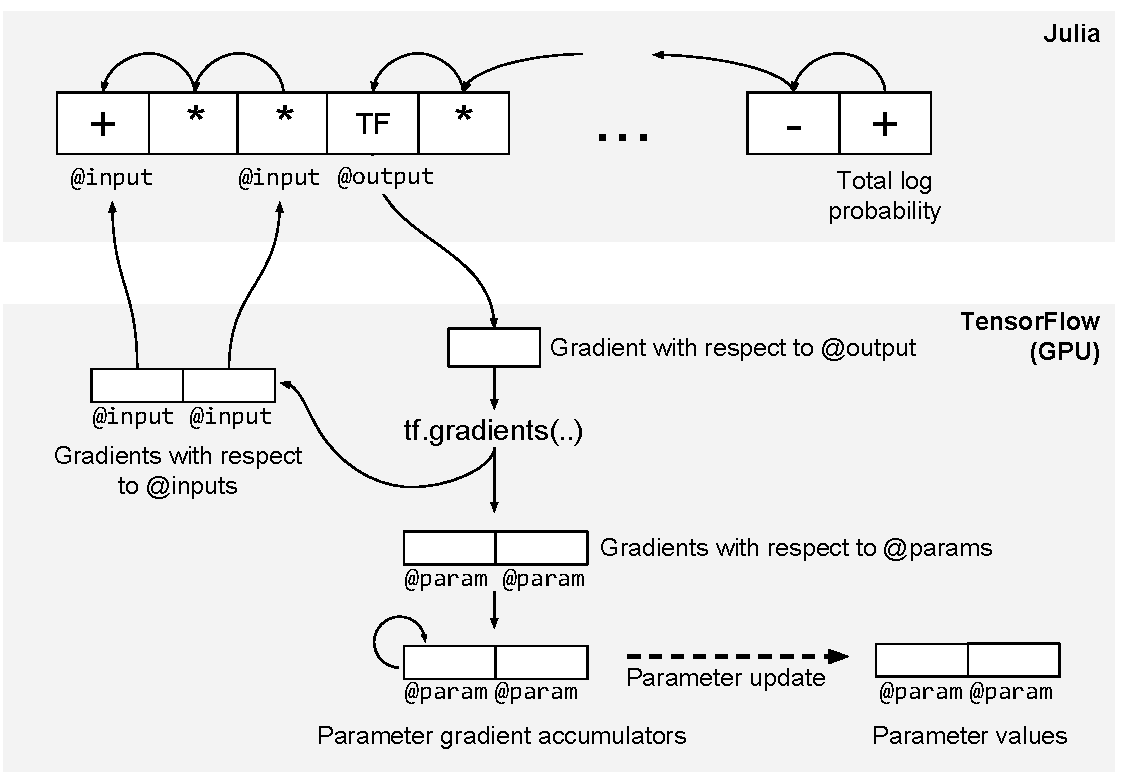
\includegraphics[width=0.7\textwidth]{images/tf-integration-schematic.pdf}
    \caption{
Reverse-mode AD in GenLite interoperates with TensorFlow functions.
A TensorFlow function produces a single element on the reverse-mode AD tape.
During the backward pass (solid lines), we receive the gradient with respect to the output (\texttt{@output}) of the TensorFlow function; TensorFlow is used to compute the gradients with respect to inputs (\texttt{@input}) and parameters (\texttt{@params}).
The gradients with respect to the parameters are accumulated across multiple backward passes, until an parameter update is performed.
A parameter update (dashed line) changes the parameter values using the accumulated gradient (in addition to any update-specific state), and resets the gradient accumulators to zero.
Parameter updates are TensorFlow operations implemented by user, defined externally from the TensorFlow function itself.
}
    \label{fig:tf-integration-schematic}
\end{figure}

\section{Combining Monte Carlo Inference and Deep Learning Proposals}
Because GenLite provides programmable inference, we can combine deep neural network proposals with other Monte Carlo strategies, like random walk moves, for refining a hypothesis.

\begin{figure}[t]
\begin{minipage}[t]{0.5\textwidth}
\begin{lstlisting}
using Cairo, ImageMagick, ImageFiltering
..

function render(glyph::Glyph)
  canvas = CairoRGBSurface(width, height)
  cc = CairoContext(canvas)
  Cairo.save(cc)

  # set background color to white
  Cairo.set_source_rgb(cc, 1.0, 1.0, 1.0)
  Cairo.rectangle(cc, 0.0, 0.0, width, height)
  Cairo.fill(cc)
  Cairo.restore(cc)
  Cairo.save(cc)

  # write the letter
  fontface = "Sans $(glyph.fontsize)"
  Cairo.set_font_face(cc, fontface)
  Cairo.text(cc, glyph.x, glyph.y, glyph.letter,
             angle=glyph.angle)

  return convert_to_png_blob(canvas)
end
\end{lstlisting}
\end{minipage}%
\begin{minipage}[t]{0.5\textwidth}
\begin{lstlisting}
model = @gen function()
  # prior
  x = width * @rand(uniform_cont(0, 1), <@\addr{"x"}@>)
  y = height * @rand(uniform_cont(0, 1), <@\addr{"y"}@>)
  size = @rand(uniform_cont(0, 1), <@\addr{"size"}@>)
  letter_id = @rand(uniform_disc(1, 3), <@\addr{"letter"}@>)
  letter = ["A", "B", "C"][letter_id]
  angle = 45 * @rand(uniform_cont(-1, 1), <@\addr{"angle"}@>)
  fontsize = scale_size(min_size, max_size, size)
  glyph = Glyph(x, y, angle, fontsize, letter)

  # render to png bytes
  image_png = render(glyph)

  # add Gaussian blur
  blur_width = 3
  blurred_png = imfilter(image_png,
                  Kernel.gaussian(blur_width))

  # add noise
  matrix = convert(Matrix{Float64}, blurred_png)
  @rand(speckle_noise(matrix, 0.1), <@\addr{"image"}@>)
end
\end{lstlisting}
\end{minipage}
\caption{Generative function for a generative model of blurry images that contain a single letter at a random location, rotation, and size. Addresses of random choices are shown in green.}
\label{fig:model-code-figure}
\end{figure}

\begin{figure}[t]
\begin{minipage}[t]{0.5\textwidth}
\begin{lstlisting}
using GenLiteTF
using TensorFlow
tf = TensorFlow

num_input = width * height
num_output = 11

function conv2d(x, W)
  tf.nn.conv2d(x, W, [1, 1, 1, 1], "SAME")
end

function max_pool_2x2(x)
  tf.nn.max_pool(x, [1, 2, 2, 1], [1, 2, 2, 1], "SAME")
end

function initial_weight(shape)
  randn(Float32, shape...) * 0.001f0
end

function initial_bias(shape)
  fill(0.1f0, shape...)
end

network = @tf_function begin

  # input image (N, 56 * 56)
  @input image_flat Float32 [-1, num_input]
  image = tf.reshape(image_flat, [-1, width, height, 1])

  # convolution + max-pooling (N, 28, 28, 32)
  @param W_conv1 initial_weight([5, 5, 1, 32])
  @param b_conv1 initial_bias([32])
  h_conv1 = tf.nn.relu(conv2d(image, W_conv1) + b_conv1)
  h_pool1 = max_pool_2x2(h_conv1)

  # convolution + max-pooling (N, 14, 14, 32)
  @param W_conv2 initial_weight([5, 5, 32, 32])
  @param b_conv2 initial_bias([32])
  h_conv2 = tf.nn.relu(conv2d(h_pool1, W_conv2) + b_conv2)
  h_pool2 = max_pool_2x2(h_conv2)
  h_pool2_flat = tf.reshape(h_pool2, [-1, 14 * 14 * 32])

  # convolution + max-pooling (N, 7, 7, 64)
  @param W_conv3 initial_weight([5, 5, 32, 64])
  @param b_conv3 initial_bias([64])
  h_conv3 = tf.nn.relu(conv2d(h_pool2, W_conv3) + b_conv3)
  h_pool3 = max_pool_2x2(h_conv3)
  h_pool3_flat = tf.reshape(h_pool3, [-1, 7 * 7 * 64])

  # fully connected layer (N, 1024)
  @param W_fc1 initial_weight([7 * 7 * 64, 1024])
  @param b_fc1 initial_bias([1024])
  h_fc1 = tf.nn.relu(h_pool3_flat * W_fc1 + b_fc1)

  # output layer (N, 11)
  @param W_fc2 initial_weight([1024, num_output])
  @param b_fc2 initial_bias([num_output])
  @output Float32 (tf.matmul(h_fc1, W_fc2) + b_fc2)
end

\end{lstlisting}
\end{minipage}%
\hfill
\begin{minipage}[t]{0.4\textwidth}
\begin{lstlisting}
predict = @gen function (outputs)

  # predict the x-coordinate
  x_mu = outputs[1]
  x_std = exp(outputs[2])
  @rand(normal(x_mu, x_std), <@\addr{"x"}@>)

  # predict the y-coordinate
  y_mu = outputs[3]
  y_std = exp(outputs[4])
  @rand(normal(y_mu, y_std), <@\addr{"y"}@>)

  # predict the rotation
  r_mu = exp(outputs[5])
  r_std = exp(outputs[6])
  @rand(normal(r_mu, r_std), <@\addr{"angle"}@>)

  # predict the size 
  size_alpha = exp(outputs[7])
  size_beta = exp(outputs[8])
  @rand(Gen.beta(size_alpha, size_beta), <@\addr{"size"}@>)
  
  # predict the identity of the letter
  log_letter_dist = outputs[9:end]
  letter_dist = exp.(log_letter_dist)
  letter_dist = letter_dist / sum(letter_dist)
  @rand(categorical(letter_dist), <@\addr{"letter"}@>)
end

proposal = @gen function ()

  # get image from input trace
  image = zeros(1, num_input)
  image[1,:] = @read(<@\addr{"image"}@>)[:]

  # run inference network
  outputs = @tf_call(network(image))

  # make prediction given inference network outputs
  @splice(predict(outputs[1,:]))
end

proposal_batch = @gen function (batch_size)

  # get images from input trace
  images = zeros(Float32, batch_size, num_input)
  for i=1:batch_size
    images[i,:] = @read((<@\addr{"\$i"}@>, <@\addr{"image"}@>))[:]
  end

  # run inference network in batch
  outputs = @tf_call(network(images))
  
  # make prediction for each image
  for i=1:batch_size
    @call(predict(outputs[i,:]), <@\addr{"\$i"}@>)
  end
end
\end{lstlisting}
\end{minipage}
\caption{
A GenLite TensorFlow (TF) function (\texttt{network}) that is invoked by a generative function (\texttt{proposal}) that implements a data-driven proposal for the model of Figure~\ref{fig:model-code-figure}.
GenLite TF functions are identified by a \texttt{@tf\_function} keyword.
The user declares inputs (\texttt{@input}, corresponding to TF placeholders), parameters (\texttt{@param}, corresponding to TF variables) and an output tensor (\texttt{@output}).
The rest of the code inside the \texttt{@tf\_function} block is regular TensorFlow code, using the TensorFlow.jl Julia wrapper \cite{?} around the TensorFlow C API.
The proposal reads the image from an input trace, runs the network, and then uses its output to parametrize distributions on the latent variables in the model.
To scalably train the network on GPU hardware, we also implement a batched variant of the proposal program, which reads from and writes to vector-shaped traces.
The batched and unbatched variants of the reuse both the TensorFlow and probabilistic prediction code.
}
\label{fig:proposal-code-figure}
\end{figure}


%x = width * @rand(uniform_cont(0, 1), <@\addr{"x"}@>)



\section{Example}

\begin{figure}[h]
\centering
    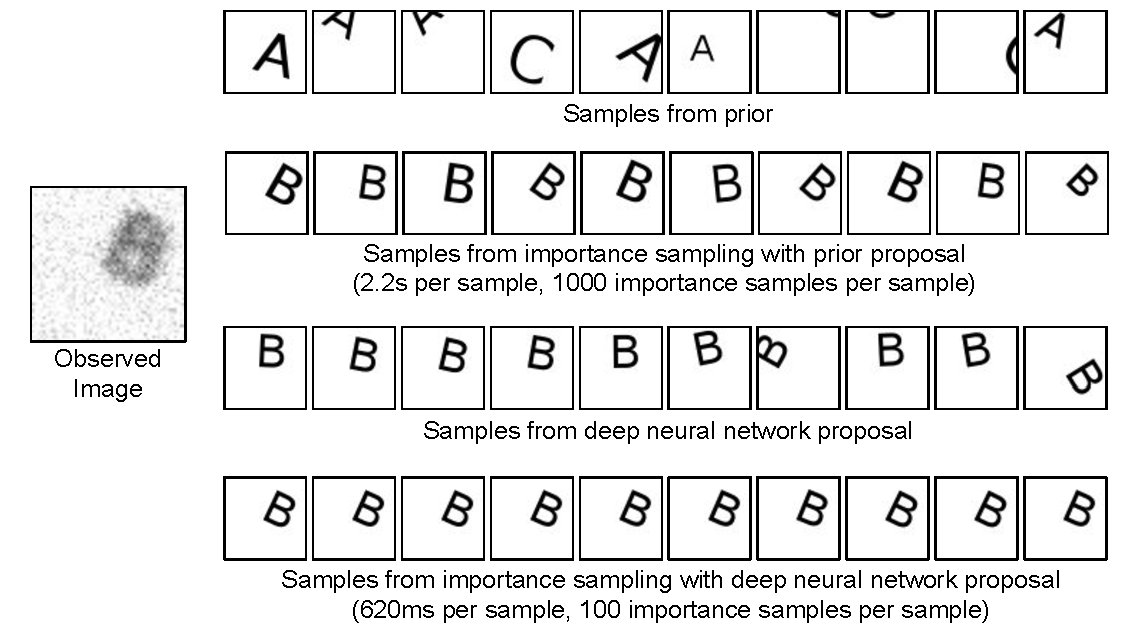
\includegraphics[width=1.0\textwidth]{images/deep-neural-network-is.pdf}
    \caption{
Inference in the generative model of Figure~\ref{fig:model-code-figure} using a combination of deep learning and model-based Monte Carlo.
On the left is the observed image, followed by a set of 10 of latent images sampled from the trained deep neural network proposal (\texttt{proposal} in Figure~\ref{fig:proposal-code-figure}), and a set of 10 latent images sampled using importance sampling, with the trained deep neural network proposal as the importance distribution.
The deep neural network was trained on traces and images jointly sampled from the generative model, using ADAM with 170,000 iterations, each with batch size 100.
The deep neural network proposal is uncertain about the location and orientiation of the letter.
Augmenting the neural network with model-based importance sampling gives more accurate inferences.
}
    \label{fig:example-results}
\end{figure}

See Figure~\ref{fig:model-code-figure}.


\section{Related Work}
Guide programs in Pyro,
Using probabilisic programs as proposals,
Edward,
Stuart Russell work on block neural proposals,
Tuan An Le's work on univeral compiled inference,
Wake sleep,
Helmholtz machines,
VAE,
Stochastic inverses

\subsubsection*{Acknowledgments}
This research was supported by DARPA (PPAML program, contract number FA8750-14-2-0004), IARPA (under research contract 2015-15061000003), the Office of Naval Research (under research contract N000141310333), the Army Research Office (under agreement number W911NF-13-1-0212), and gifts from Analog Devices and Google.
This research was conducted with Government support under and awarded by DoD, Air Force Office of Scientific Research, National Defense Science and Engineering Graduate (NDSEG) Fellowship, 32 CFR 168a.

\bibliographystyle{unsrtnat}
\bibliography{references}

\end{document}
